\documentclass[11pt,a4paper]{scrartcl} %scrartcl from KOMA-script uses sans headers and looks less latexy than article
%\usepackage[doublespacing]{setspace}
%\usepackage[capposition=top]{floatrow} %for notes under pics
%\usepackage[nomarkers]{endfloat}
\usepackage{natbib}
\usepackage[utf8]{inputenc}
%\usepackage{amsmath}
%\usepackage{amsfonts}
%\usepackage{amssymb}
\usepackage[left=2.5cm,right=2.5cm,top=3cm,bottom=3cm]{geometry}
\usepackage[pdftex, hidelinks]{hyperref}
\usepackage{graphicx}
\usepackage{grffile}
\usepackage{booktabs}
\usepackage[blocks]{authblk} %for affil
\usepackage{url}
\usepackage{tabularx}
\usepackage{csvsimple}
\usepackage[nomessages]{fp}
\usepackage{enumitem}
\setlist{noitemsep} % \setlist{nosep} to reove separation around lists as well


%citation cheat sheet:
	%\cite{key}					Jones et al. (1990)
	% \citet{key}				Jones et al. (1990)
	% \citet*{key}				Jones, Baker, and Smith (1990)
	% \citep{key}				(Jones et al. 1990)
	% \citep*{key}				(Jones, Baker, and Smith 1990)
	% \citep[p.~99]{key}		(Jones et al., 1990, p. 99)
	% \citep[e.g.][]{key}		(e.g. Jones et al., 1990)
	% \citep[e.g.][p.~99]{key}	(e.g. Jones et al., 1990, p. 99)
	% \citeauthor{key}			Jones et al.
	% \citeauthor*{key}			Jones, Baker, and Smith
	% \citeyear{key}			1990
	% \citealt{key} 			Jones et al. 1990


\newcommand{\figureloc}{C:/Users/Koen/Dropbox/PhD/Papers/CongoGBV/Figures}
\newcommand{\tableloc}{C:/Users/Koen/Dropbox/PhD/Papers/CongoGBV/Tables}
\newcommand{\bibloc}{C:/Users/Koen/Dropbox/Literatuur/Mendeley/Bibtex/CongoGBV}





\begin{document}

\author{Koen Leuveld}

\affil{Development Economics Group, Wageningen University \\
\href{mailto:koen.leuveld@wur.nl}{koen.leuveld@wur.nl}}



\title{Sexual Violence in Eastern DRC}
\subtitle{Exploratory evidence from a list experiment} %needs scrartcl

\maketitle

%\begin{abstract}
%Abstract to come
%\end{abstract}


%%%%%%%%%%%%%%%%%%%%%%%%%%
\section*{Introduction}
%%%%%%%%%%%%%%%%%%%%%%%%%

\paragraph{}
%Hook
Eastern DR Congo has been called the "rape capital of the world". Much of this has been linked to the decades of violence that the region has seen over the past decades. Various armed groups have used Gender Based Violence (GBV) as a weapon against the population. This has put the issue on the radar of the international community. Today, most of the NGOs operating in the region focus on GBV, either exclusively, or as part of broader programmes. The 2018 Nobel Peace prize was awarded to Dr. Denis Mukwege, for his work on victims of GBV at Bukavu's Panzi Hospital.

\paragraph{}
%Research question
The issue of GBV is complicated. While the armed conflict is universally seen as a large driver of GBV, customs and tradition leave Congolese women in a powerless position. This paper aims to provide quantitative evidence on the correlates of sexual violence.

\paragraph{}
%Antecedents
Antecedents of this paper include (perhaps weave this in with contribution):

GBV in Congo: \\
\textbf{The role of conflict in GBV}: \cite{Porter2019} argues that conflict shapes what behaviour is acceptable. In this way, conflict may have an effect on the degree to which women experience GBV. \\%weakly doe.

\cite{Autesserre2012a} argues that this focus on the role of sexual violence in the conflict in the DRC has been counter-productive, as it has distracted attention from other pressing problems the country faces.	\cite{Hilhorst2018} agree that the focus on the role of conflict in GBV (rape as a weapon of war) constituted a hype. However, they do note the local aid landscape has evolved from treating conflict victims, to improving the general conditions of women, even in peacetime, while the international narrative has remained focus on rape. \\
	%citeer ook: 
	%Kirby, P. (2015) ‘Ending sexual violence in conflict: the preventing sexual violence initiative and its critics’. International Affairs. 91(3). pp. 457–472.
	%Bouta, T., G. Frerks, and I. Bannon (2005) Gender, Conflict and Development. The World Bank, Washington, DC
	%Peterman, A., T. Palermo, and C. Bredenkamp (2011) ‘Estimates and determinants of sexual violence against women in the Democratic Republic of Congo’. American Journal of Public Health. 101(6).pp. 1060–1067.
	%Maria Eriksson Baaz and Maria Stern, ‘The complexity of violence: a critical analysis of sexual violence in the Democratic Republic of Congo (DRC)’ (SIDA and the Nordic Africa Institute, Stockholm, 2010), pp. 15–16 and 59
\textbf{Other determinants of GBV}: In a study where 87 women and girls in South Kivu were interviewed using Audio Assisted Self-Interviews (ACASI) techniques, \citet{Stark2017} find that 14\% of respondents reported having been victim of sexual coercion. Half of these were perpetrated by the respondents' husbands or boyfriends. Crucially, in complementary group discussions, respondents did not bring up intimate partners at all. This points at the difficulties of collecting accurate data about GBV. \\
%include papers cited by stark on the role of intimate partners in conflict settings.
	
\textbf{Female empowerment in Congo}: In Congolese society, women hold an inferior position. For example, views that men have the right to physically abuse their wife if she is disobedient are broadly held \citep{Quattrochi2019}. \\
%add papers cited by Johny boy.

%\cite{Hilhorst2018}:  question whether the reponse of the international community should be labelled a hype.
%\cite{Quattrochi2019}: "Empowerment programs often target women who have survived sexual and gender-basedviolence (SGBV), with the justification that these women may develop disempowered beliefs as a copingmechanism, or face greater barriers to, or derive greater benefits from, the adoption of empowered beliefs andpreferences."
%\cite{Porter2019}: argues that rape as a weapon of war is not helpful. It is embedded in existing mores and customs. 
%close to my paper: \cite{Stark2017} assess disclosement bias.
%	\item List experiment literature: 
%Classic example: The 1991 National Race and Politics Survey (\cite{Sniderman1991}). Used to measure racial prejudice. Recently, more of of them have been done. \cite{Imai2011}: introduction of new estimator. \cite{Blair2012}: overview of literature. \cite{Tsai2019}: implement methods in Stata.


\paragraph{}
%Contribution
While from the literature it is obvious that GBV is endemic in Eastern Congo, it is difficult to get quantitative evidence on the problem. The area is poorly accessible to research teams, and women may be unwilling to divulge information on victimization due to the stigma involved. We collected data in the region in 2014, as part of the evaluation of Dutch development efforts. The questionnaire included a section on gender. As part of this section, a list experiment was administered.

\paragraph{}
%Road Map


%%%%%%%%%%%%%%%%%%%%%%%%%%%%%%%%
\section*{Background and data}
%%%%%%%%%%%%%%%%%%%%%%%%%%%%%%%%
\paragraph{}
%to do in this section: desctibe N.varlabels
The data for this study was collected as part of an evaluation of Dutch development aid in 2014. This evaluation concerned projects ran by three NGOs in the territories of Fizi and Uvira in South Kivu province. A household survey formed part of this evaluation. The final module of this survey dealt with gender issues, and was administered to an adult female in the household.  To collect data on the sensitive topic of GBV, this module contained a list experiment. For this, the respondents were randomly divided into two groups. Each group was presented with a number of issues that women can realistically face in Eastern Congo. They then indicated how many of the issues they themselves had faced. The first group (Control) was presented with the following issues:
\begin{itemize}
	\item Lack of food;
	\item Lack of money;
	\item Theft; and,
	\item Sterility.
\end{itemize}

\paragraph{}
 Women in the second group (Treatment) were presented with the same four items, but a fifth item was added: Sexual Violence. While this means I cannot know who among our respondents was the victim of GBV, I can compare the means of the number of issues between the groups to arrive at an estimate of GBV. By comparing means between sub-samples, and by using more sophisticated methods proposed by \citet{Imai2011} (and implemented by \cite{Tsai2019} in Stata), I can find the correlates of GBV. 

 \paragraph{}
 In addition to the list experiment, I conducted a household bargaining game based on \cite{Martinsson2009}. In this, couples choose between a set of six risky lotteries, based on \cite{Holt2002}; first individually, then jointly. The lotteries presented range from fairly low-risk ones -- where low and high pay-out are nearly equal -- to high-risk one, with a large difference between high and low pay-outs. By comparing the couple decision with the individual decision, I obtain an indicator for barganing power. Specifically, I divide the women in three groups: where the joint decision is closer to the woman's decision, where the joint decision is equally far from both decisions, and where the joint decision is closest to the husband's.

\paragraph{}
Table \ref{tab:balance} presents descriptive statistics of the sample. Our sample consists of 508 married women. Their a

%consider using csvsimple or DataTools to import this,
\begin{table}[hp] \centering
\newcolumntype{C}{>{\centering\arraybackslash}X}

\caption{Descriptive statistics by treatment assignemt}
\label{tab:balance}
{\footnotesize
\begin{tabularx}{\linewidth}{lCCCCCCC}

\toprule
&{(1)}&{(2)}&{(3)}&{(4)}&{(5)}&{(6)}&{(7)} \tabularnewline
&\multicolumn{2}{c}{All}&\multicolumn{2}{c}{Treatment}&\multicolumn{2}{c}{Control}&{(4)-(6)}\tabularnewline \midrule
{}&{N}&{Mean}&{N}&{Mean}&{N}&{Mean}&{ } \tabularnewline
\midrule \addlinespace[\belowrulesep]
Number of reported issues&593&2.49&291&2.65&302&2.34&0.30*** \tabularnewline
&&(0.94)&&(1.03)&&(0.83)& \tabularnewline
Conflict pre-2012: property lost&530&0.77&264&0.79&266&0.75&0.04 \tabularnewline
&&(0.42)&&(0.41)&&(0.43)& \tabularnewline
Conflict pre-2012: HH member killed&530&0.49&264&0.51&266&0.48&0.03 \tabularnewline
&&(0.50)&&(0.50)&&(0.50)& \tabularnewline
Conflict 2013--2014: Viol. against civilians&496&6.73&239&6.68&257&6.77&--0.08 \tabularnewline
&&(4.69)&&(4.70)&&(4.69)& \tabularnewline
Family MR had more land&450&0.33&224&0.33&226&0.33&--0.00 \tabularnewline
&&(0.47)&&(0.47)&&(0.47)& \tabularnewline
Family FR had more land&450&0.21&224&0.22&226&0.19&0.02 \tabularnewline
&&(0.41)&&(0.41)&&(0.40)& \tabularnewline
Bargaining: choice Female Respondent&593&3.58&291&3.59&302&3.56&0.04 \tabularnewline
&&(2.06)&&(2.08)&&(2.05)& \tabularnewline
Barganing: choice Male Respondent&184&3.45&97&3.49&87&3.40&0.09 \tabularnewline
&&(2.14)&&(2.12)&&(2.18)& \tabularnewline
Bargaining: closer to MR&184&0.40&97&0.37&87&0.44&--0.07 \tabularnewline
&&(0.49)&&(0.49)&&(0.50)& \tabularnewline
Bargaining: closer to FR&184&0.27&97&0.32&87&0.21&0.11* \tabularnewline
&&(0.44)&&(0.47)&&(0.41)& \tabularnewline
Age of FR&593&41.09&291&40.49&302&41.67&--1.17 \tabularnewline
&&(14.01)&&(14.06)&&(13.96)& \tabularnewline
Age of MR&449&45.67&224&44.48&225&46.85&--2.37** \tabularnewline
&&(13.80)&&(13.09)&&(14.40)& \tabularnewline
HH Head Female&593&0.26&291&0.24&302&0.27&--0.03 \tabularnewline
&&(0.44)&&(0.43)&&(0.45)& \tabularnewline
FR completed primary education&593&0.25&291&0.26&302&0.25&0.01 \tabularnewline
&&(0.44)&&(0.44)&&(0.43)& \tabularnewline
FR completed secondary education&593&0.03&291&0.02&302&0.04&--0.02 \tabularnewline
&&(0.17)&&(0.13)&&(0.20)& \tabularnewline
MR completed primary education&449&0.63&224&0.63&225&0.63&0.01 \tabularnewline
&&(0.48)&&(0.48)&&(0.48)& \tabularnewline
MR completed secondary education&449&0.20&224&0.19&225&0.20&--0.01 \tabularnewline
&&(0.40)&&(0.39)&&(0.40)& \tabularnewline
Household has a tin roof&593&0.61&291&0.62&302&0.59&0.03 \tabularnewline
&&(0.49)&&(0.49)&&(0.49)& \tabularnewline
Household owns livestock&593&0.49&291&0.51&302&0.47&0.03 \tabularnewline
&&(0.50)&&(0.50)&&(0.50)& \tabularnewline
territory==Uvira&593&0.24&291&0.24&302&0.23&0.01 \tabularnewline
&&(0.43)&&(0.43)&&(0.42)& \tabularnewline
territory==Fizi&593&0.63&291&0.65&302&0.62&0.03 \tabularnewline
&&(0.48)&&(0.48)&&(0.49)& \tabularnewline
Project Beneficary&593&0.50&291&0.49&302&0.50&--0.01 \tabularnewline
&&(0.50)&&(0.50)&&(0.50)& \tabularnewline
\bottomrule \addlinespace[\belowrulesep]

\end{tabularx}
\begin{flushleft}
\footnotesize FR = Female Respondent; MR = Male Respondent; Standard Deviations in parentheses; *p $<$ 0.1,**p $<$ 0.05,***p $<$ 0.01
\end{flushleft}
}
\end{table}



%some examples on how to interpret list experiments:
%\cite{Meng2017} run various types of models. Consistently refer to mean difference models, and Maximum Likelihood models

%\cite{Blair2014}: extremely detailed stuff. Thread carefully!
%\cite{Frye2017} simple difference in means model.

%%%%%%%%%%%%%%%%%%%%%%%%%%%%%%%%
\section*{Results}
%%%%%%%%%%%%%%%%%%%%%%%%%%%%%%%%
%build up the story a bit more:
%	* Average incidence; include graphs of mean differences?
%	* Present some sample splits in this figure as well: conflict; marriage types.
%	* Present full models

%	* Present sample splits: married before conflict vs. married after conflict. 
%	* Sexual Violence can come from a number of sources. Salient in the DRC is conflict-related GBV.
%	
%
%	* Is there difference for women married "after" the war vs. before the war?


%command to get incidences from csv file
\newcommand{\incid}[2]{\csvreader[filter strcmp={\key}{#1}]{\tableloc/incidence.csv}{key=\key,#2=\inc}{\inc}}

\paragraph{}
First, I compare the number of issues faced by the two groups of women. The difference between the group who were presented with only four issues (the control group) and the group who were presented four issues plus GBV (the treatment group) is my estimate of the incidence of GBV. The average number of issues reported by the control group is \incid{overall1}{mean0}, while the number if issues reported by the treatment group is \incid{overall1}{mean1} (see Figure \ref{fig:meancompare_overall}). The difference of \incid{overall1}{incidence} implies that the incidence of GBV is \incid{overall1}{incidence_pct}\% in this sample. The p-value for a t-test on this difference is \incid{overall1}{p}. This incidence is slightly higher than some estimates \citep{Quattrochi2019}.

\begin{figure}
  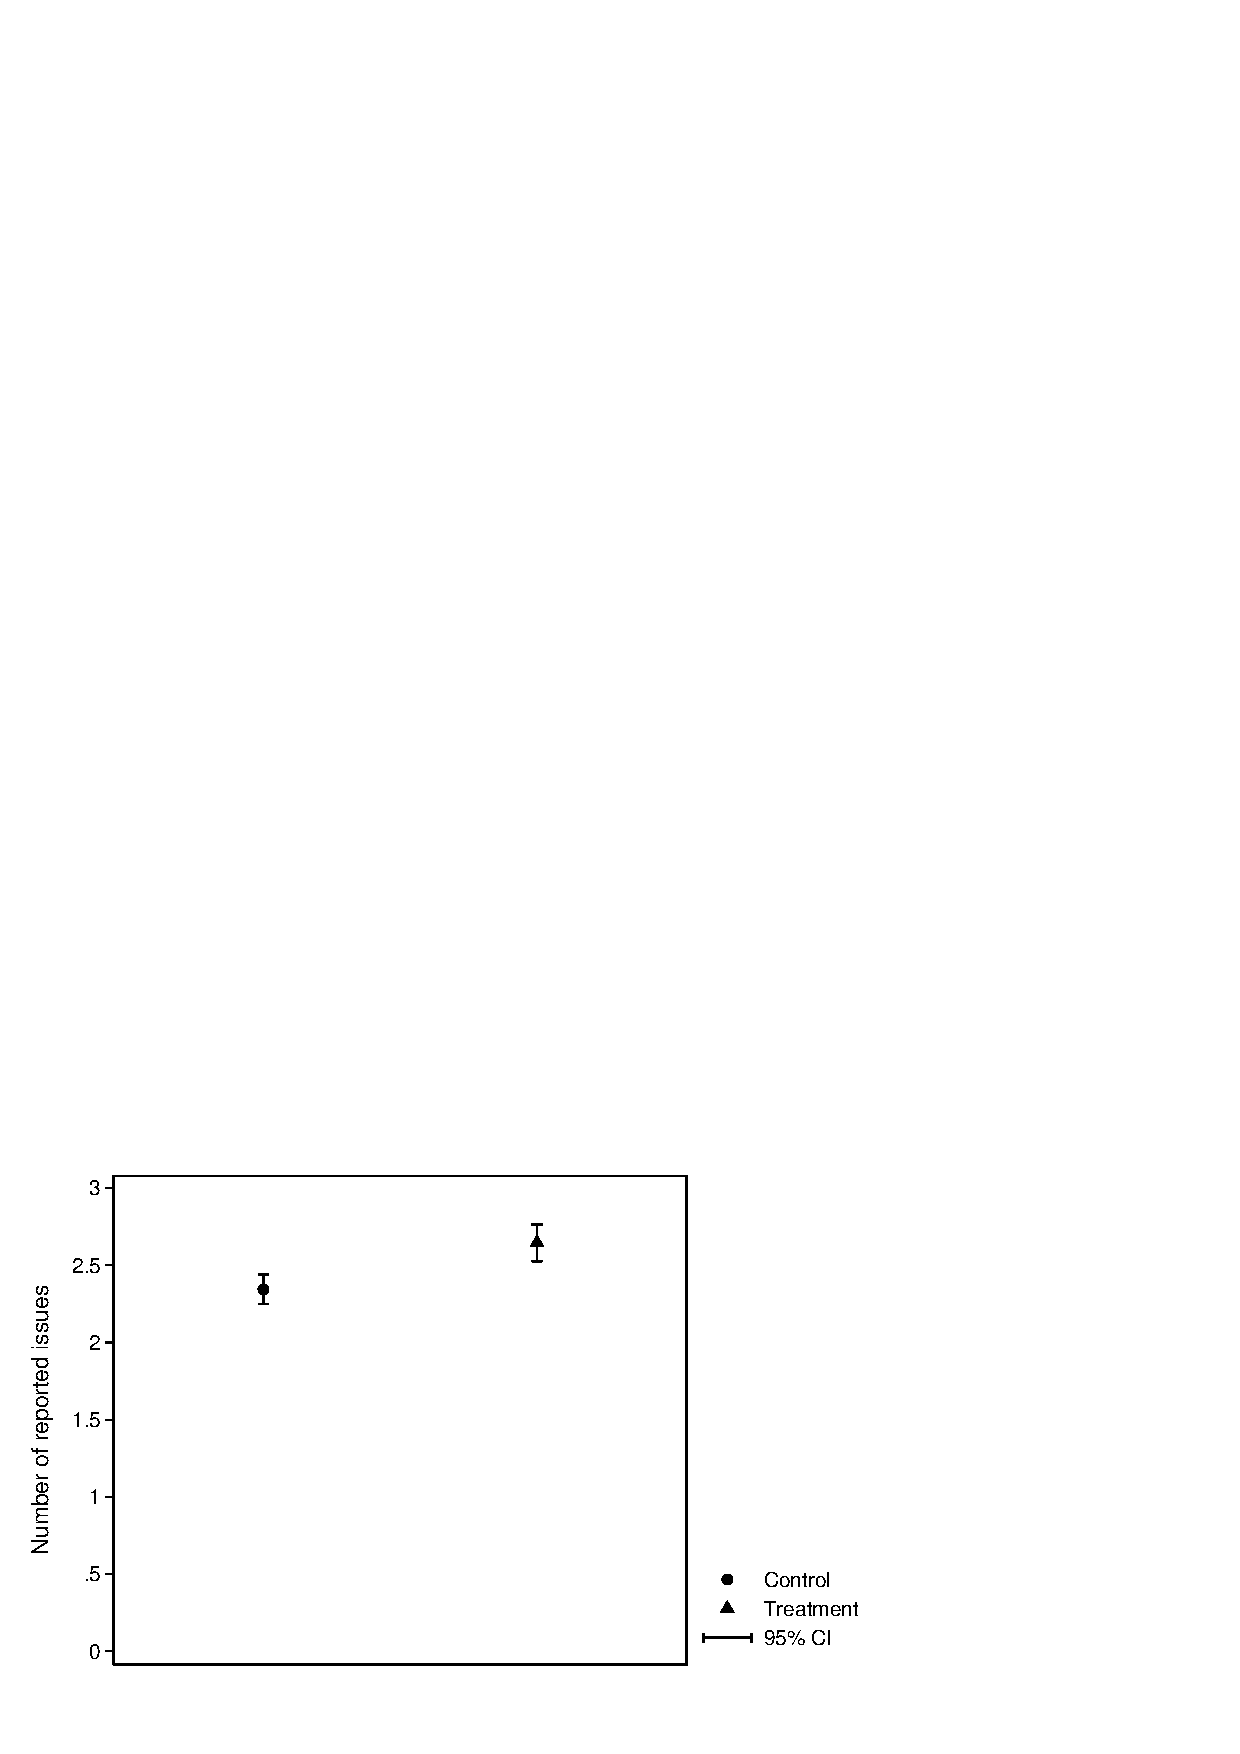
\includegraphics[width=0.8\linewidth]{\figureloc/meancompare_overall.png}
  \caption{Comparison of means of issues faced: treatment vs. control.}
  \label{fig:meancompare_overall}
\end{figure}

\subsection*{Intra-household dynamics}
\paragraph{}
I then compare the number of issues faced in several sub-groups. First, I focus on marriage dynamics. I compare women across the relative status of the partners at the time of marriage. For this, I use the land held by the partners' families as proxy for status (figure \ref{fig:meancompare_mar1}). Given the importance of agriculture, and conversely land, in the study area, this is a reasonably proxy. In the group where the wife had more status before the marriage (n=\incid{statpar1}{n}), the average number of issues was \incid{statpar1}{mean0} for the control group, and \incid{statpar1}{mean1} for the treatment group. The difference in means implies a rate of GBV of \incid{statpar1}{incidence_pct} (p-value of a t-test on the means = \incid{statpar1}{p}). In the group where the partners were of equal standing (n=\incid{statpar2}{n}), the average number of issues was \incid{statpar2}{mean0} for the control group, and \incid{statpar2}{mean1} for the treatment group. This implies a rate of GBV of \incid{statpar2}{incidence_pct} (p = \incid{statpar2}{p}). In the group where the husband had more status (n=\incid{statpar3}{n}), the average number of issues was \incid{statpar3}{mean0} for the control group, and \incid{statpar3}{mean1} for the treatment group. This implies a rate of GBV of \incid{statpar3}{incidence_pct} (p = \incid{statpar3}{p}).

\begin{figure}
  \includegraphics[width=0.8\linewidth]{\figureloc/meancompare_mar1.png}
  \caption{Comparison of means of issues faced by pre-marriage status.}
  \label{fig:meancompare_mar1}
\end{figure}

\paragraph{}
The second intra-household aspect I explore is derived from the results of a bargaining game played with couples. Couples first took a decision individually, and then jointly. I then create three groups, based on whether the joint decision is closer to the husband's decision, to the wife's, or if the distance is equal. See figure \ref{fig:meancompare_mar2}. In the group where the couple decision was closest to the wife's decision (n=\incid{bargresult1}{n}), the average number of issues was \incid{bargresult1}{mean0} for the control group, and \incid{bargresult1}{mean1} for the treatment group. This implies a rate of GBV of \incid{bargresult1}{incidence_pct}\% (p = \incid{bargresult1}{p}). In the group where the couple decision was equally close to the husband and wife (n=\incid{bargresult2}{n}), the average number of issues was \incid{bargresult2}{mean0} for the control group, and \incid{bargresult2}{mean1} for the treatment group. This implies a rate of GBV of \incid{bargresult2}{incidence_pct}\% (p = \incid{bargresult2}{p}). In the group where the couple decision was closest to the husband's (n=\incid{bargresult3}{n}), the average number of issues was \incid{bargresult3}{mean0} for the control group, and \incid{bargresult3}{mean1} for the treatment group. This implies a rate of GBV of \incid{bargresult3}{incidence_pct}\% (p = \incid{bargresult3}{p}).

\begin{figure}
  \includegraphics[width=0.8\linewidth]{\figureloc/meancompare_mar2.png}
  \caption{Comparison of means of issues faced: forced marriage vs. other marriage types.}
  \label{fig:meancompare_mar2}
\end{figure}


\paragraph{}
The final intra-household variable I use to compare women, is their relative contribution to the household's cash income (see figure \ref{fig:meancompare_mar3}). The household questionnaire collected data on all activities of household members, and what the contribution of these activities were to household income. I sum this for all activities for the women in the sample, and compare those who contribute more than 50\% of cash income with those who do not. In the group where the woman does not contribute more than 50\% of cash income (n=\incid{contribcashyn0}{n}), the average number of issues was \incid{contribcashyn0}{mean0} for the control group, and \incid{contribcashyn0}{mean1} for the treatment group. This implies a rate of GBV of \incid{contribcashyn0}{incidence_pct}\% (p = \incid{contribcashyn0}{p}). In the group where the woman does contribute more than 50\% of cash income (n=\incid{contribcashyn1}{n}), the average number of issues was \incid{contribcashyn1}{mean0} for the control group, and \incid{contribcashyn1}{mean1} for the treatment group. This implies a rate of GBV of \incid{contribcashyn1}{incidence_pct}\% (p = \incid{contribcashyn1}{p}). 

\begin{figure}
  \includegraphics[width=0.8\linewidth]{\figureloc/meancompare_mar3.png}
  \caption{Comparison of means of issues faced across contribution to cash income.}
  \label{fig:meancompare_mar3}
\end{figure}


\subsection*{Conflict}
I then compare the conflict history of the respondents' households, to assess whether conflict victimization correlates with the incidence of GBV. I use data collected from an earlier round of the study that collected detailed conflict exposure data. First, I compare respondents who live in households who have suffered loss of (or damage to) property, including agricultural fields, due to conflict. See \ref{fig:meancompare_conf1}. In the non-victimized group (n=\incid{victimproplost0}{n}), the average number of issues was \incid{victimproplost0}{mean0} for the control group, and \incid{victimproplost0}{mean1} for the treatment group. This implies a rate of GBV of \incid{victimproplost0}{incidence_pct}\% (p = \incid{victimproplost0}{p}). For the group that has suffered loss of property due to the conflict (n=\incid{victimproplost1}{n}), the average number of issues was \incid{victimproplost1}{mean0} for the control group, and \incid{victimproplost1}{mean1} for the treatment group. This implies a rate of GBV of \incid{victimproplost1}{incidence_pct}\% (p = \incid{victimproplost1}{p}).

\begin{figure}
  \includegraphics[width=0.8\linewidth]{\figureloc/meancompare_conf1.png}
  \caption{Comparison of means of issues faced across conflict exposure.}
  \label{fig:meancompare_conf1}
\end{figure}

The second conflict indicator I examine, is whether the respondent's household has lost any household members or family as a consequence of the conflict.See \ref{fig:meancompare_conf2}. In the non-victimized group (n=\incid{victimfamlost0}{n}), the average number of issues was \incid{victimfamlost0}{mean0} for the control group, and \incid{victimfamlost0}{mean1} for the treatment group. This implies a rate of GBV of \incid{victimfamlost0}{incidence_pct}\% (p = \incid{victimfamlost0}{p}). For the group that has suffered loss of property due to the conflict (n=\incid{victimfamlost1}{n}), the average number of issues was \incid{victimfamlost1}{mean0} for the control group, and \incid{victimfamlost1}{mean1} for the treatment group. This implies a rate of GBV of \incid{victimfamlost1}{incidence_pct}\% (p = \incid{victimfamlost1}{p}).

\begin{figure}
  \includegraphics[width=0.8\linewidth]{\figureloc/meancompare_conf2.png}
  \caption{Comparison of means of issues faced across conflict exposure.}
  \label{fig:meancompare_conf2}
\end{figure}

\subsection*{Assets}
I then explore the relationship between asset holdings and GBV. The first asset I consider, is having a tin roof (figure \ref{fig:meancompare_ses1}). These roofs are a substantial improvement over thatch roofs, but about half the sample doesn't own them. This makes for a simple, yet non-arbitrary, way to split the sample in richer and poorer households.   In the group without tin roofs (n=\incid{tinroof0}{n}), the average number of issues was \incid{tinroof0}{mean0} for the control group, and \incid{tinroof0}{mean1} for the treatment group. This implies a rate of GBV of \incid{tinroof0}{incidence_pct}\% (p = \incid{tinroof0}{p}). For the group with tin roofs (n=\incid{tinroof1}{n}), the average number of issues was \incid{tinroof1}{mean0} for the control group, and \incid{tinroof1}{mean1} for the treatment group. This implies a rate of GBV of \incid{tinroof1}{incidence_pct}\% (p = \incid{tinroof1}{p}).

\begin{figure}
  \includegraphics[width=0.8\linewidth]{\figureloc/meancompare_ses1.png}
  \caption{Comparison of means of issues faced across asset holdings (tin roof).}
  \label{fig:meancompare_ses1}
\end{figure}

\paragraph{}
A second asset with important status implications for the household is livestock (see figure \ref{fig:meancompare_ses2}).  In the group without livestock (n=\incid{livestockany0}{n}), the average number of issues was \incid{livestockany0}{mean0} for the control group, and \incid{livestockany0}{mean1} for the treatment group. This implies a rate of GBV of \incid{livestockany0}{incidence_pct}\% (p = \incid{livestockany0}{p}). For the group with tin roofs (n=\incid{livestockany1}{n}), the average number of issues was \incid{livestockany1}{mean0} for the control group, and \incid{livestockany1}{mean1} for the treatment group. This implies a rate of GBV of \incid{livestockany1}{incidence_pct}\% (p = \incid{livestockany1}{p}).

\begin{figure}
\includegraphics[width=0.8\linewidth]{\figureloc/meancompare_ses2.png}
  \caption{Comparison of means of issues faced across asset holdings (livestock).}
  \label{fig:meancompare_ses2}
\end{figure}

\paragraph{}
In summary, I find that women who are in a disadvantageous position in their household, either because they are of lower status, or because they have less bargaining power, are more likely to have experienced GBV. The results with respect to conflict were ambiguous, and I find no suggestion that respondents in poorer household experience GBV at a higher rate than their peers in richer households. If anything, I find the opposite. There are two large caveats with these findings: (i) they are not causal; (ii) by running separate comparisons, any conclusions are at risk of missing variable bias. While the first one is hard to address using list experiments, it is possible to come to more rigourous estimates of effects than presented so far. 

\paragraph{}
In table \ref{tab:results_regression} I display the results of a number of regressions. These are linear regressions: the coefficients reported should be interpreted as the marginal effects on the difference between control and treatment (i.e. the interaction between the variable and the treatment indicator). For brevity, the level effects of each variable on the total number of issues is omitted, as these coefficients are not of interest here. In the first column, I report the results of including only endline survey measures; in the second, I add baseline conflict indicators; in the third I include results from the bargaining game. Finally, I estimate a full model. I find that neither conflict exposure, nor household asset holdings are correlated to the incidence of GBV. Intra-household dynamics on the other hand, are strongly correlated to GBV. Nearly all the GBV happens to women who live in male dominated households. From this, we cannot conclude that it is the husbands who perpetrate the violence. It may be possible that both GBV, and choosing partners of high status, are both determined by the same factors. However, contrary to popular narratives, we find no evidence of correlation to conflict exposure.

\newcommand{\coeffget}[3]{\csvreader[filter=\equal{\reg}{#1} \and \equal{\var}{#2}]{\tableloc/regs.csv}{var=\var,reg=\reg,#3=\coeff}{\coeff}}
%TEST: \coeffget{l1}{Delta:husbmoreland}{coef}

\begin{table}
	\caption{Results}\label{tab:results_regression}
	\begin{center}
	{
\def\sym#1{\ifmmode^{#1}\else\(^{#1}\)\fi}
\begin{tabular}{l*{4}{c}}
\hline\hline
                    &\multicolumn{1}{c}{(1)}   &\multicolumn{1}{c}{(2)}   &\multicolumn{1}{c}{(3)}   &\multicolumn{1}{c}{(4)}   \\
\hline
Family MR had more land&       0.419** &               &               &       0.451*  \\
                    &     (0.204)   &               &               &     (0.240)   \\
[1em]
Conflict pre-2012: HH member killed&               &       0.409** &               &       0.374** \\
                    &               &     (0.182)   &               &     (0.179)   \\
[1em]
Conflict 2013-2014: Viol. against civilians&               &               &      0.0120   &      0.0147   \\
                    &               &               &    (0.0224)   &    (0.0230)   \\
[1em]
FR empowerment attitudes&               &               &               &    0.000101   \\
                    &               &               &               &    (0.0199)   \\
[1em]
Age of FR           &     0.00843   &     0.00684   &     0.00563   &      0.0110   \\
                    &    (0.0161)   &    (0.0182)   &    (0.0186)   &    (0.0207)   \\
[1em]
Age of MR           &     -0.0122   &    -0.00929   &    -0.00778   &     -0.0111   \\
                    &    (0.0149)   &    (0.0162)   &    (0.0174)   &    (0.0189)   \\
[1em]
HH Head Female      &     0.00951   &     -0.0766   &       0.257   &       0.421   \\
                    &     (0.445)   &     (0.525)   &     (0.318)   &     (0.410)   \\
[1em]
FR completed secondary education&      -1.111***&      -1.347***&      -1.034***&      -1.249***\\
                    &     (0.320)   &     (0.351)   &     (0.336)   &     (0.332)   \\
[1em]
MR completed primary education&     -0.0390   &     -0.0655   &      -0.193   &      -0.263   \\
                    &     (0.166)   &     (0.178)   &     (0.181)   &     (0.177)   \\
[1em]
Household has a tin roof&       0.292   &       0.279   &       0.184   &       0.214   \\
                    &     (0.203)   &     (0.221)   &     (0.234)   &     (0.233)   \\
[1em]
Household owns livestock&     -0.0455   &    -0.00342   &      -0.142   &      -0.193   \\
                    &     (0.160)   &     (0.181)   &     (0.177)   &     (0.186)   \\
[1em]
territory==Uvira    &       0.418   &       0.202   &       0.438   &       0.205   \\
                    &     (0.264)   &     (0.342)   &     (0.288)   &     (0.360)   \\
[1em]
territory==Fizi     &       0.511*  &       0.232   &       0.504*  &       0.191   \\
                    &     (0.292)   &     (0.365)   &     (0.302)   &     (0.379)   \\
[1em]
Project Beneficary  &      0.0542   &      0.0121   &      0.0382   &      0.0732   \\
                    &     (0.163)   &     (0.177)   &     (0.157)   &     (0.167)   \\
[1em]
Constant            &      -0.162   &    -0.00267   &    -0.00290   &      -0.111   \\
                    &     (0.483)   &     (0.506)   &     (0.491)   &     (0.614)   \\
\hline
Observations        &         449   &         402   &         379   &         350   \\
\hline\hline
\end{tabular}
}

	\end{center}
\end{table}

%interpretatie voorbeelden:
%\cite{Meng2017} first simply present mean differences; they then present a maximum likelihood model. Based on this model, they predict mean differences and present this as their quantity of interest. They have replication files online.

%\cite{Imai2011}: himself admits that the coefficients of the maximum likelihood method are difficult to compare. He therefore generates predicted values of shares of people answering affirmitively to the sensitive item for two subgroups.

%\cite{Bulte2019}: how they do interpret.


%bibliography, this is needed for bibtex
\clearpage 
\bibliographystyle{chicago}
%path to .bib file (e.g. automatically exported by mendeley) exclude the file extension!
\bibliography{\bibloc}

\end{document}
